\documentclass[12pt,a4paper,titlepage]{article}
%\usepackage[T1]{fontenc}
\usepackage{fontspec}
\usepackage[margin=3cm]{geometry}
\usepackage{textcomp}
\usepackage{titlesec}
\usepackage{fancyhdr}
\usepackage{fix-cm}
\usepackage{graphicx}
\usepackage{etoolbox}
\usepackage{xcolor}
\usepackage{float}
\usepackage{ifthen}
\usepackage{multicol}
\usepackage{minted}
\usepackage{pgfplots}
\usepackage{etoolbox}
\usepackage[group-separator={'}]{siunitx}
\usepackage{tablefootnote}
\usepackage[margin=1cm]{caption}
\usepackage[bottom,marginal]{footmisc}
\usepackage[breaklinks=true]{hyperref}
\usepackage{cleveref}
\usepackage[backend=biber,style=numeric,natbib=true,sorting=none]{biblatex}
\usepackage[bachelorthesis]{systems-cover/systems-cover}
\usepackage{pdfpages}
\pagestyle{fancy}
\setlength{\headheight}{30pt}
\renewcommand{\arraystretch}{1.5}
\newmintinline[code]{text}{}
\setminted{breaklines=true,fontsize=\footnotesize,autogobble=true}
\setmonofont{Consolas}

\hypersetup{
  colorlinks,
  linkcolor={darkgray},
  citecolor={blue!50!black},
  urlcolor={blue!80!black}
}

\providecommand*{\listingautorefname}{listing}

\covernum{197b}
\covertitle{Implementation of a Benchmark Suite for Strymon}
\coverauthor{Nicolas Hafner}
\coverdate{November 2017 - May 2018}
\coversupervisedby{Dr.\ John Liagouris \\ Prof.\ Timothy Roscoe}

\addbibresource{content/references.bib}

\setcounter{biburllcpenalty}{7000}
\setcounter{biburlucpenalty}{8000}
\DeclareFieldFormat*{citetitle}{#1}
\DeclareFieldFormat{formaturl}{\newline #1}
\newbibmacro*{url+urldate}{%
  \printtext[formaturl]{%
    \printfield{url}}%
  \iffieldundef{urlyear}
  {}
  {\setunit*{\addspace}%
    \printtext[urldate]{\printurldate}}}

\newcommand{\citefulltitle}[1]{\citetitle*{#1}\cite{#1}}

\newcommand{\imagefigure}[3][]{\begin{figure}[H]%
    \centering%
    \includegraphics[width=1.0\linewidth]{#2}%
    \caption{#3}%
    \ifthenelse{ \equal{#1}{} }%
    {}%
    {\label{figure:#1}}%
  \end{figure}}

\usetikzlibrary{
  pgfplots.colorbrewer,
}
\pgfplotsset{
  % define a `cycle list' for marker
  cycle list/.define={my marks}{
    every mark/.append style={solid,fill=\pgfkeysvalueof{/pgfplots/mark list fill}},mark=*\\
    every mark/.append style={solid,fill=\pgfkeysvalueof{/pgfplots/mark list fill}},mark=square*\\
    every mark/.append style={solid,fill=\pgfkeysvalueof{/pgfplots/mark list fill}},mark=triangle*\\
    every mark/.append style={solid,fill=\pgfkeysvalueof{/pgfplots/mark list fill}},mark=diamond*\\
  },
}

\pgfplotsset{tikzDefaults/.style=
  {legend pos=outer north east,
    ymajorgrids=true,
    grid style=dashed,
    cycle list/Spectral-11,
    cycle multiindex* list={
      Spectral-11
      \nextlist
      my marks
      \nextlist
      [3 of]linestyles
      \nextlist
      very thick
      \nextlist},
  }}

\makeatletter
\newcommand{\latencyplot}[3]{%
  \begin{tikzpicture}
    \begin{axis}[
      tikzDefaults,
      title={Median Latency (#1 workers)},
      ylabel={Rate [e/s]},
      xlabel={Latency [s]},
      xmode=log, ymode=log,
      x tick label style={/pgf/number format/fixed},
      ]
      
      \forcsvlist{\latencyplot@item{#1}}{#2}
      \ifthenelse{ \equal{#3}{} }{}{\legend{#3}}
    \end{axis}
  \end{tikzpicture}}

\newcommand{\latencyplot@item}[2]{%
  \addplot table[y index=0, x index=#2] {data/latency-#1.csv};%
}

\newcommand{\scalingplot}[3]{%
  \begin{tikzpicture}
    \begin{axis}[
      tikzDefaults,
      title={Scaling (\num{#1} e/s)},
      xlabel={Workers [n]},
      ylabel={Latency [s]},
      xmode=log,
      log basis x={2},
      scaled y ticks=false,
      y tick label style={/pgf/number format/fixed},
      xtick={1, 2, 4, 8, 16, 32},
      ]
      
      \forcsvlist{\scalingplot@item{#1}}{#2}
      \ifthenelse{ \equal{#3}{} }{}{\legend{#3}}
    \end{axis}
  \end{tikzpicture}}

\newcommand{\scalingplot@item}[2]{%
  \addplot table[x index=0, y index=#2] {data/scaling-#1.csv};%
}

\newcommand{\cdfplot}[4]{%
  \begin{tikzpicture}
    \begin{axis}[
      tikzDefaults,
      title={CDF (#1 workers, \num{#2} e/s)},
      xlabel={Latency [s]},
      ylabel={CDF [\%]},
      xmode=log,
      ]
      
      \forcsvlist{\cdfplot@item{#1}{#2}}{#3}
      \ifthenelse{ \equal{#4}{} }{}{\legend{#4}}
    \end{axis}
  \end{tikzpicture}}

\newcommand{\cdfplot@item}[3]{%
  \addplot table[skip first n=1, y index=0, x index=#3] {data/cdf-#1-#2.csv};%
}

\newcommand{\ccdfplot}[4]{%
  \begin{tikzpicture}
    \begin{axis}[
      tikzDefaults,
      title={CCDF (#1 workers, #2 e/s)},
      xlabel={Latency [s]},
      ylabel={CCDF [\%]},
      xmode=log, x dir=reverse
      ]
      
      \forcsvlist{\cdfplot@item{#1}{#2}}{#3}
      \ifthenelse{ \equal{#4}{} }{}{\legend{#4}}
    \end{axis}
  \end{tikzpicture}}

\makeatother

\newcommand{\latencyfigure}[4][]{\begin{figure}[H]%
    \centering
    \latencyplot{#2}{#3}{#4}%
    \caption{Loglog plot of the benchmark's rate behaviour for #2 workers.}%
    \ifthenelse{ \equal{#1}{} }%
    {}%
    {\label{figure:#1-latency}}%
  \end{figure}}

\newcommand{\scalingfigure}[4][]{\begin{figure}[H]%
    \centering
    \scalingplot{#2}{#3}{#4}%
    \caption{Linlog plot of the benchmark's scaling behaviour for \num{#2} e/s.}%
    \ifthenelse{ \equal{#1}{} }%
    {}%
    {\label{figure:#1-scaling}}%
  \end{figure}}

\newcommand{\cdffigure}[5][]{\begin{figure}[H]%
    \centering
    \cdfplot{#2}{#3}{#4}{#5}%
    \caption{Cumulative distribution function plot of the benchmark's latency behaviour for #2 workers and \num{#3} e/s.}%
    \ifthenelse{ \equal{#1}{} }%
    {}%
    {\label{figure:#1-cdf}}%
  \end{figure}}

\newcommand{\ccdffigure}[5][]{\begin{figure}[H]%
    \centering
    \ccdfplot{#2}{#3}{#4}{#5}%
    \caption{Complementary cumulative distribution function plot of the benchmark's latency behaviour #2 workers and #3 e/s.}%
    \ifthenelse{ \equal{#1}{} }%
    {}%
    {\label{figure:#1-ccdf}}%
  \end{figure}}

\setcounter{secnumdepth}{4}
\titleformat{\paragraph}{\normalfont\normalsize\bfseries}{\theparagraph}{1em}{}
\titlespacing*{\paragraph}{0pt}{3.25ex plus 1ex minus .2ex}{1.5ex plus .2ex}

\newcommand{\tb}[1]{\textbf{#1}}
\newcommand{\ti}[1]{\textit{#1}}

\begin{document}
\begin{abstract}
  Over recent years the amount of recorded and observed data has increased massively. Many systems are now dealing with enormous volumes of data and continuous streams of new data arriving in real-time. This change in trends has prompted a need for systems that are capable of dealing with such hard real-time, large volume constraints. \\

  A multitude of such systems have been developed, each with their own focus areas, strengths, and weaknesses. One such system under development at ETH is Strymon, based on Timely Dataflow. \\
  
  In this thesis we survey a number of papers on streaming data processing systems and assess their evaluation experiments. We also implement three major benchmarks that have found application in the industry: the Yahoo Streaming Benchmark, Intel's HiBench, and the NEXMark benchmark. We briefly evaluate the results of the implementations of these benchmarks for the Timely system. Finally, we discuss important points that need to be addressed for the formulation of a future benchmark for streaming systems.
\end{abstract}

%%% Local Variables:
%%% mode: latex
%%% TeX-master: "../thesis"
%%% TeX-engine: luatex
%%% End:

\renewcommand{\abstractname}{Acknowledgements}
\begin{abstract}
  I would like to thank the entire DCModel group at ETH for making this thesis a thoroughly enjoyable and pleasant experience. Everyone has been exceedingly nice and helpful, and I felt comfortable and welcome at all times. \\

  \noindent I am especially thankful to my supervisor, Dr. John Liagouris, for all the support he has given me throughout the thesis' work. He has been essential in keeping things on track, and in helping me resolve the various problems and hurdles that came up over time. \\

  \noindent I would also like to specifically thank Dr. Frank McSherry for offering me a lot of his valuable time to explain and help discuss various aspects of the Timely system. \\

  \noindent Finally I would like to thank Prof. Timothy Roscoe for allowing me to work on a thesis with a group of such excellent people.
\end{abstract}

%%% Local Variables:
%%% mode: latex
%%% TeX-master: "../thesis"
%%% TeX-engine: luatex
%%% End:

\tableofcontents\newpage
\section{Introduction}

%%% Local Variables:
%%% mode: latex
%%% TeX-master: "../thesis"
%%% TeX-engine: luatex
%%% TeX-command-extra-options: "-shell-escape"
%%% End:

\section{Preliminaries}
\subsection{Data Flow Essentials}
Many algorithms can be conveniently formulated as a data flow --- a directed graph whose nodes represent operations performed on data, and whose edges represent the flow of data between such operators. This representation is especially handy for streaming systems, where the data is continuously fed into the system. Most of the streaming data processing systems in use today make use of data flows as the primary programming mechanism. Users express their programs in the form of several operators that are connected together, forming the \ti{logical data flow}. The system then turns this logical data flow into a \ti{physical data flow} by distributing the computation across \ti{workers}. Workers represent physical processing units such as the cores of a processor, or individual machines in a network. \\

\imagefigure[dataflow]{images/dataflow.pdf}{An illustration of the difference between logical (top) and physical (bottom) data flows. This illustration is based on the Timely model, where each operator specifies how the data it receives in the physical data flow should be redistributed between workers. The map operator for instance does not request redistribution of the data.}

The data to be processed by each operator is distributed to each worker by the system, though the precise mechanisms of this vary with each system. Often the data is partitioned into disjoint sets, and each worker is assigned one set of this data. After the worker has completed the operator's work, the generated output data is passed on to the next operator and might be redistributed across the workers.

\subsection{Timely Dataflow}
Timely\cite{timely} is a system written in Rust based on research initially proposed in Naiad\cite{naiad}. Timely offers a dataflow based processing framework, where a dataflow is composed of a possibly cyclic graph of operators. Each operator can receive data from previous operators through input edges in the graph, and send data to other operators through output edges. Each edge represents a communication channel that is managed by the Timely system, which allows parallelising the computation to many workers at a time. Timely handles the exchange of data between operators and across workers. \\

Timely tracks progress of the dataflow computation through ``epochs'' --- rounds of input data that are associated with a logical timestamp. These timestamps are required to implement a partial order, which is used to infer information about the progress of an operator. An important part of this inference is the notion of epoch closure: when an epoch is closed, no more input may arrive for it. Operators can request to be notified when specific epochs are closed, and can thus reason about when they have the full picture of the data. As a consequence of this, data before the closure of an epoch can arrive out of order, which typically improves performance as it lowers synchronisation constraints. The tracking of the epoch closure is called the ``frontier''. \\

The permission of cycles in the dataflow graph is achieved through ``scopes''. Any cycle must be encapsulated by such a scope. Each scope extends the timestamp by another dimension that tracks the progress within that scope. When the scope receives notification that an epoch has closed, it then continues processing until all inner epochs have been closed as well, at which point it can advance the frontier itself and propagate the information to the operators after the scope as well. \\

While the physical exchange of data is handled by Timely itself, data is only sent to other workers if requested, either by an explicit exchange operator, or by the communication contract specified by an operator. This allows the implementer of an operator to decide whether it makes sense to re-distribute the processing of the data. For instance, a keyed reduction would profit from having the data set partitioned over the workers according to the keys. A simple map on the other hand would not profit from having its data bucketed over the workers first.

%%% Local Variables:
%%% mode: latex
%%% TeX-master: "../thesis"
%%% TeX-engine: luatex
%%% TeX-command-extra-options: "-shell-escape"
%%% End:

%% FIXME: Note what state is retained for each stateful operator
\section{Related Work}
In this section we analyse and compare a number of papers about stream processors. In particular, we look at the ways in which they evaluate and test their systems in order to get an idea of how benchmarking has so far commonly been done. Each subsection looks at one paper at a time, providing a graph of the data flows and operators used to evaluate the system, if such information was available. \\

Operators in the data flow graphs are coloured in orange if they retain state over multiple records. \\

The papers were selected based on the number of citations, as well as on their direct relevance to current trends in the development and research for Big Data and streaming systems. \\

Overall we found that most of the systems were evaluated with relatively simple data flows and algorithms that are well understood. A lot of the papers also do not provide direct source code, nor a way to replicate the workload to confirm their findings. It seems that so far no generally accepted algorithm, workload, setup, nor even a precisely defined way of measuring performance have emerged.

\subsection{\citetitle*{s4}}
The S4 paper\cite{s4} evaluates its performance with two algorithms: click-through rate (CTR), and online parameter optimisation (OPO). \\

\imagefigure{images/s4-graphs.pdf}{Graphs of the two data flows used to evaluate the S4 platform: click-through rate (top) and online parameter optimisation (bottom).}

The CTR data flow is implemented by four operators: initially a map assigns key to the keyless events coming in. It passes them to a operator that combines matching events. From there the events go on to a filter that removes unwanted events. Finally, the events are passed to a operator that computes the CTR, and emits it as a new event. \\

The OPO data flow consists of five operators: the split operator assigns keys to route the events to either one of the map operators. These operators then perform some computations on the events and emit the results as new events. The reduce operator compares the events it gets in order to determine the optimisation parameters. The final map operator runs an adaptation depending on the parameters it receives and passes them onwards.

\subsection{\citetitle*{spade}}
In order to evaluate the system, the paper\cite{spade} employs a simple data flow to determine bargains to buy. \\

\imagefigure{images/spade-graphs.pdf}{Graph of the example used in the SPADE paper: a bargain index computation.}

The data flow is composed of six operators: a filter operator filters out trade information and computes its price. It passes its information on to a moving reduce operator, with a window size of 15 tuples, and a slide of 1 tuple. The reduction result is passed on to a mapping operator that computes the volume weighted average price (VWAP). Another filter operator filters out quote information from the main input stream. This is then, together with the VWAP, reduced to compute the bargain index. The final filter simply removes the zero indexes.

\subsection{\citetitle*{discretized}}
In the Discretized Streams paper\cite{discretized}, the performance is evaluated through a simple Word Count algorithm. \\

\imagefigure{images/discretized-graphs.pdf}{Graph of the Word Count example used to illustrate the discretized streams.}

The Word Count data flow is implemented through three operators: a ``flat map'' that splits an incoming string into words, a map that turns each word into a tuple of the word and a counter, and finally a tumbling window reduction that adds the counters together grouped by word.

\subsection{\citetitle*{millwheel}}
The Millwheel paper\cite{millwheel} unfortunately provides barely any information at all about the data flows implemented. The only mention is about how many stages the pipelines have they use to evaluate the system. Two tests are performed: a single-stage data flow to measure the latency, and a three-stage data flow to measure the lag of their fault tolerance system.

\subsection{\citetitle*{streamcloud}}
In this paper\cite{streamcloud}, the system is evaluated by two distinct data flows. It is not stated whether either of the data flows have any real-world application. The StreamCloud system provides a number of predefined operators that can be strung together to perform these data flows. \\

\imagefigure{images/streamcloud-graphs.pdf}{Graph of the data flows used to evaluate StreamCloud.}

Both data flows perform a sequence of maps and filters followed by reductions. The reduction is based on a window size and slide, which can be configured for each operator. However, the configurations used are not provided by the paper.

\subsection{\citetitle*{integrating}}
To evaluate their approach for fault tolerance using Operator State Management\cite{integrating}, two data flows were implemented: a linear road benchmark (LRB) to determine tolls in a network, and a Top-K data flow to determine the top visited pages. The data flow is composed out of stateless and stateful operators, where stateful operators must communicate their state to the system so that it may be recovered. \\

\imagefigure{images/integrating-graphs.pdf}{Illustration of the data flows for the Linear Road Benchmark (top) and Top-K (bottom) used to evaluate their system.}

The LRB is implemented using six operators. The first split operator routes the tuples depending on their type. The following map operator calculates tolls and accidents, the information of which is then forwarded to a operator that collects toll information, and a operator that evaluates the toll information. The output from the evaluation, together with account balance information, is aggregated and finally reduced to a single tuple together with the information from the toll collector operator. \\

The Top-K data flow is implemented using three operators. The starting map operator strips unnecessary information from the tuples. The following operator reduces the tuples to local top-k counts. Finally the many local counts are reduced to a single top-k count for the whole data.

\subsection{\citetitle*{timestream}}
The TimeStream system\cite{timestream} is evaluated using two algorithms: a distinct count to count URLs and a Twitter sentiment analysis. \\

\imagefigure{images/timestream-graphs.pdf}{The Distinct Count (top) and Sentiment Analysis (bottom) data flows used to evaluate the Timestream system.}

The distinct count is implemented using five operators. The split operator distributes the tuples based on a hash. The following filter removes bot-generated data flows, and passes them on to a windowing operator with a window of 30 seconds and a slide of 2 seconds. The windowed events are then reduced into local counts. The local counts are finally reduced into global counts. \\

The sentiment analysis performs two individual computations before finally joining the results together with a custom operator. The first computation determines changes in sentiments. It uses a tumbling window on the tweets, averages the sentiments, for each window, then uses a sliding window of 2 ms to feed a filter that only returns sentiments that changed. The second computation returns the change in word counts. It uses a tumbling window of the same size as the first computation, then reduces the word counts for each batch. Using another sliding window of 2 ms it then computes a delta in the counts. Using a custom operator the sentiment changes and word count deltas are then joined together to analyse them.

\subsection{\citetitle*{storm}}
This paper proposes a new scheduling algorithm for Storm. It then uses a data flow specifically geared towards evaluating the scheduling. This data flow is believed to be representative of typical topologies found in applications of Storm.\\

\imagefigure{images/storm-graphs.pdf}{The topology graph used to evaluate the Storm schedulers.}

The data flow is composed of a sequence of operators that produce arbitrary, new events distinguished by a counter. The data flow has no interesting properties aside from the alternation between stateless and stateful operators.

\subsection{\citetitle*{storm2}}
This paper\cite{storm2} presents a case study to perform real-time analysis of trends on Twitter using Storm. \\

\imagefigure{images/storm2-graphs.pdf}{An illustration of the topology used for the Twitter \& Bitly link trend analysis.}

The data flow for this is the most complicated one presented in the related works we analysed. It uses a total of eleven operators, excluding edge operators that act as interfaces to the external systems. The computation can be separated into three stages: Twitter extraction, Bit.ly extraction, and trend analysis. The first stage filters out tweets that contain Bit.ly links. Those are then sent to the Bit.ly extraction stage and a map that extracts useful values for the trend analysis. The second stage extracts relevant information from the Bit.ly feed, then uses this together with the code received from the first stage to perform a Bloom filter. The output from there is then filtered for useful values before being saved. The trend analysis uses the extracted values from the tweets to find hashtags, which are then put through a rolling-window count. The resulting counts are reduced by two stages of ranking.

\subsection{\citetitle*{bigdatabench}}
This paper\cite{bigdatabench} proposes a suite of benchmarks and tests to evaluate Big Data systems. The paper primarily focuses on the generation of suitable testing data sets, and proposes the following algorithms to test the system:

\begin{multicols}{2}
  \begin{itemize}
  \item Sort
  \item Grep
  \item Word Count
  \item Retrieving Data
  \item Storing Data
  \item Scanning Data
  \item Select Query
  \item Aggregate Query
  \item Join Query
  \item Nutch Server
  \item Indexing
  \item Page Rank
  \item Olio Server
  \item K-means
  \item Connected Components
  \item Rubis Server
  \item Collaborative Filtering
  \item Naive Bayes
  \end{itemize}
\end{multicols}

The paper does not propose any particular implementation strategies. They provide performance evaluation for an implementation of different parts of the benchmark suite on the Hadoop, MPI, Hbase, Hive, and MySQL systems, but no particular details of the implementation are discussed.

\subsection{Comparison}
In \autoref{table:test-properties} and \autoref{table:test-setups} we compare the most important features of the tests performed in the various papers. We also include the three benchmarks we discuss in detail in the following sections. Unfortunately, most of the papers do not supply or use publicly available data, making it difficult to compare them, even if the data flows were replicated.

\begin{table}[H]
  \centering
  {
    \scriptsize
    \hspace*{-1cm}
    \begin{tabular}{|p{3cm}|p{4cm}|p{3cm}|p{2.5cm}|p{2.5cm}|}
      \hline
      \tb{Paper} & \tb{Goal} & \tb{Application} & \tb{Data Flow Properties} & \tb{Data Flow Operators}
      \\\hline
      
      S4\cite{s4}
      & A practical application of the system to a real-life problem.
      & Search
      & Stateful, DAG
      & Map, Filter, Join
      \\\hline
      
      SPADE\cite{spade}
      & Sample application, performance study.
      & Finance
      & Stateful, DAG
      & Map, Filter, Window Reduce, Join
      \\\hline

      D-Streams\cite{discretized}
      & Scalability and recovery test.
      & None
      & Chain
      & Map, Window Reduce
      \\\hline

      Millwheel\cite{millwheel}
      & In-Out Latency.
      & Ads
      & Unspecified
      & Unspecified
      \\\hline

      StreamCloud\cite{streamcloud}
      & Evaluation of scalability and elasticity.
      & Telephony
      & Stateful, Chain
      & Map, Filter, Window Reduce
      \\\hline

      Seep\cite{integrating}
      & Testing dynamic scaling and fault-tolerance.
      & Road tolls
      & Stateful, DAG
      & Map, Reduce, Join
      \\\hline

      TimeStream\cite{timestream}
      & Low-latency test for real-world applications.
      & Search, Social Network
      & DAG
      & Map, Filter, Reduce, Join, Window
      \\\hline

      Adaptive Scheduling\cite{storm}
      & Evaluating performance of scheduling algorithms.
      & None
      & Stateful, Chain
      & Reduce
      \\\hline

      Analytics on High Velocity Streams\cite{storm2}
      & Analysing trends for links on Twitter.
      & Social Network
      & Stateful, DAG
      & Map, Filter, Reduce, Join, Window
      \\\hline

      BigDataBench\cite{bigdatabench}
      & Fair performance evaluation of big data systems.
      & Search, Social, Commerce
      & Unspecified
      & Unspecified
      \\\hline

      YSB\cite{ysb}
      & Benchmarking streaming systems via Ad analytics.
      & Ads
      & Stateful
      & Map, Filter, Reduce, Join, Window
      \\\hline

      HiBench\cite{hibench}
      & Evaluating big data processing systems.
      & Big Data
      & Stateful
      & Map, Reduce, Window
      \\\hline

      NEXMark\cite{nexmark}
      & Adaptation of XMark for streaming systems.
      & Auctioning
      & Stateful
      & Map, Filter, Reduce, Join, Window, Session
      \\\hline
    \end{tabular}
  }
  \caption{Comparison of the test properties of the reference papers.}
  \label{table:test-properties}
\end{table}

%% FIXME: Clarify whether workloads are generated or real data sets.
\begin{table}[H]
  \centering
  {
    \scriptsize
    \hspace*{-1cm}
    \begin{tabular}{|p{3cm}|p{3.5cm}|p{4cm}|p{2.5cm}|p{2cm}|}
      \hline
      \tb{Paper} & \tb{Workloads} & \tb{Testbed} & \tb{External Systems} & \tb{Public Data}
      \\\hline
      
      S4\cite{s4}
      & \textasciitilde 1M live events per day for two weeks.
      & 16 servers with 4x32-bit CPUs, 2GB RAM each.
      & Unspecified
      & No
      \\\hline
      
      SPADE\cite{spade}
      & \textasciitilde 250M transactions, resulting in about 20GB of data.
      & 16 cluster operators. Further details not available.
      & IBM GPFS
      & Maybe\tablefootnote{The data was retrieved from the IBM WebSphere Web Front Office for all of December 2005.}
      \\\hline

      D-Streams\cite{discretized}
      & \textasciitilde 20 MB/s/operator (200K records/s/operator) for WordCount.
      & Up to 60 Amazon EC2 operators, 4 cores, 15GB RAM each.
      & Unspecified
      & No
      \\\hline

      Millwheel\cite{millwheel}
      & Unspecified.
      & 200 CPUs. Nothing further is specified.
      & BigTable
      & No
      \\\hline

      StreamCloud\cite{streamcloud}
      & Up to 450'000 transactions per second.
      & 100 operators, 32 cores, 8GB RAM, 0.5TB disks each, 1Gbit LAN.
      & Unspecified
      & No
      \\\hline

      Seep\cite{integrating}
      & Up to 600'000 tuples/s.
      & Up to 50 Amazon EC2 ``small'' instances with 1.7GB RAM.
      & Unspecified
      & No
      \\\hline

      TimeStream\cite{timestream}
      & \textasciitilde 30M URLs, \textasciitilde 1.2B Tweets.
      & Up to 16 Dual Xeon X3360 2.83GHz, 8GB RAM, 2TB disks each, 1Gbit LAN.
      & Unspecified
      & No
      \\\hline

      Adaptive Scheduling\cite{storm}
      & Generated.
      & 8 operators, 2x2.8GHz CPU, 3GB RAM, 15GB disks each, 10Gbit LAN.
      & Nimbus, Zookeper
      & Yes\tablefootnote{The data is generated on the fly, the algorithm of which is specified in the paper.}
      \\\hline

      Analytics on High Velocity Streams\cite{storm2}
      & \textasciitilde 1'600GB of compressed text data.
      & 4 operators, Intel i7-2600 CPU, 8GB RAM each.
      & Kafka, Cassandra
      & Maybe\tablefootnote{Data stems from Twitter and Bit.ly for June of 2012, but is not publicly available.}
      \\\hline

      BigDataBench\cite{bigdatabench}
      & Up to 1TB.
      & 15 operators, Xeon E5645, 16GB RAM, 8TB disks each.
      & Hadoop, MPI, Hbase, Hive, MySQL
      & Yes\tablefootnote{Obtainable at \url{http://prof.ict.ac.cn/BigDataBench/}}
      \\\hline

      YSB\cite{ysb}
      & Generated
      & Unspecified
      & Kafka, Redis
      & Yes\tablefootnote{Generated by YSB: \url{https://github.com/yahoo/streaming-benchmarks}}
      \\\hline

      HiBench\cite{hibench}
      & Generated
      & Unspecified
      & Kafka
      & Yes\tablefootnote{Generated by HiBench.}
      \\\hline

      NEXMark\cite{nexmark}
      & Generated
      & Unspecified
      & Firehose Stream Generator
      & Yes\tablefootnote{Generated by the ``Firehose Stream Generator''.}
      \\\hline

    \end{tabular}
  }
  \caption{Comparison of the test setups of the reference papers.}
  \label{table:test-setups}
\end{table}

%%% Local Variables:
%%% mode: latex
%%% TeX-master: "../thesis"
%%% TeX-engine: luatex
%%% TeX-command-extra-options: "-shell-escape"
%%% End:

\section{Benchmark Framework}
In order to factor out common operations and to be able to cleanly define the data flows of each test in the benchmarks we developed a small framework. This framework takes care of processing command line arguments, Timely setup, and statistical data collection. All that's necessary in order to implement a benchmark is the implementation of the \code{Benchmark} trait for the overall benchmark, and the implementation of the \code{TestImpl} trait for each test in the benchmark.

\begin{listing}[H]
\begin{minted}{rust}
pub trait Benchmark {
    fn name(&self) -> &str;
    fn generate_data(&self, config: &Config) -> Result<()>;
    fn tests(&self) -> Vec<Box<Test>>;
}
\end{minted}
  \caption{Definition of the Benchmark trait.}
  \label{lst:benchmark-trait}
\end{listing}

The \code{Benchmark} includes a method to generate input data files that can be used to feed into the system from disk at a later point, and a function to return all the tests that the benchmark defines. Note that it returns \code{Test} trait instances rather than \code{TestImpl}. This is done to avoid leaking associated trait types into surrounding code that doesn't need to know about it.

\begin{listing}[H]
\begin{minted}{rust}
pub trait Test : Sync+Send {
    fn name(&self) -> &str;
    fn run(&self, config: &Config, worker: &mut Root<Generic>)
        -> Result<Statistics>;
}
\end{minted}
  \caption{Definition of the Test trait.}
  \label{lst:test-trait}
\end{listing}

The \code{Test} trait includes only one important method, which runs the test on a given worker and returns collected statistical data of the run if it completed was successfully. The \code{Test} trait is automatically implemented for all types that implement the \code{TestImpl} trait, thus avoiding the need to manually implement the \code{Test} trait, and automatically erasing the associated types required in the \code{TestImpl} definition.

\begin{listing}[H]
\begin{minted}{rust}
pub trait TestImpl : Sync+Send {
    type D: Data;
    type DO: Data;
    type T: Timestamp;

    fn name(&self) -> &str;
    fn create_endpoints(&self, &Config, index: usize, workers: usize)
        -> Result<(Source<Self::T, Self::D>, Drain<Self::T, Self::DO>)>;
    fn construct_dataflow<'scope>(&self, &Config, stream: 
          &Stream<Child<'scope, Root<Generic>, Self::T>, Self::D>)
        -> Stream<Child<'scope, Root<Generic>, Self::T>, Self::DO>;
    fn run(&self, &Config, worker: &mut Root<Generic>)
        -> Result<Statistics>;
}
\end{minted}
  \caption{Definition of the TestImpl trait.}
  \label{lst:testimpl-trait}
\end{listing}

The \code{TestImpl} trait is the most complicated, but should not be hard to utilise either. The \code{run} method has a default implementation and as such typically does not need to be implemented. This implementation makes use of the associated \code{D}, \code{DO}, and \code{T} types in order to work regardless of the test's type requirements. The \code{create_endpoints} method is responsible for initialising the input and output of the data flow. This method is required to be implemented in order for the test to function properly, but should be very straight-forward.

\begin{listing}[H]
\begin{minted}{rust}
 fn create_endpoints(&self, config: &Config, _: usize, _: usize)
    -> Result<(Source<Self::T, Self::D>, Drain<Self::T, Self::DO>)> {
     Ok((Source::from_config(config,
           Source::new(Box::new(NEXMarkGenerator::new(config))))?,
         Drain::from_config(config)?))
 }
\end{minted}
  \caption{A sample definition of the \code{create_endpoints} method.}
  \label{lst:create-endpoints}
\end{listing}

Finally, the most important method is \code{construct_dataflow}. It is responsible for transforming the input data stream into an output data stream, implementing the data flow logic. The function bodies of the respective \code{construct_dataflow} implementations are shown in the Data Flows subsections of each Benchmark.

\subsection{Additional Operators}
In order to ease the implementation of the benchmarks and improve the usability of the Timely system we introduced a number of additional operators. We will outline and discuss these operators here shortly.

\subsubsection{FilterMap}
This operator performs a filter followed by a map in one go. The operator expects a closure which can choose to either filter events by returning \code{None}, or map them by returning \code{Some(..)} with the output data.

\begin{listing}[H]
\begin{minted}{rust}
fn filter_map(&self, map) -> Stream {
    self.unary_stream(move |input, output| {
        input.for_each(|time, data| {
            let mut session = output.session(time);
            data.for_each(|x|{
                if let Some(d) = map(x) {
                    session.give(d);
                }
            });
        });
    })
}
\end{minted}
  \caption{Simplified code for the filter map operator.}
  \label{lst:filtermap}
\end{listing}

The operator is mostly useful for streams that contain multiple types of data encapsulated in an enum. In that case turning the stream into one of a single type is trivial using \code{filter_map}.

\begin{listing}[H]
\begin{minted}{rust}
enum Vehicle {
    Car(Car)
    Boat(Boat)
}

impl Car { 
    fn from(vehicle: Vehicle) -> Option<Car> {
        match vehicle {
            Vehicle::Car(car) => Some(car),
            _ => None
        }
    }
}

stream.filter_map(|x| Car::from(x))
\end{minted}
\caption{An example of the filter map operator to purify a stream of vehicles into one of cars.}
\label{lst:filtermap-example}
\end{listing}

\subsubsection{Join}
This operator offers two forms of joins that merge two separate streams of data into one. The first is an epoch based join, meaning data is only matched up between the two streams within a single epoch. If no match is found for either stream, the data is discarded.

\begin{listing}[H]
\begin{minted}{rust}
fn epoch_join(&self, stream, key_1, key_2, joiner) -> Stream{
    let mut epoch1 = HashMap::new();
    let mut epoch2 = HashMap::new();
    
    self.binary_notify(move |input1, input2, output, notificator| {
        input1.for_each(|time, data|{
            let epoch = epoch1.entry(time).or_insert_with(HashMap::new);
            data.for_each(|dat|{
                let key = key_1(&dat);
                let datavec = epoch.entry(key).or_insert_with(Vec::new);
                datavec.push(dat);
            });
            notificator.notify_at(time);
        });
        
        input2.for_each(|time, data|{
            let epoch = epoch2.entry(time).or_insert_with(HashMap::new);
            data.for_each(|dat|{
                let key = key_2(&dat);
                let datavec = epoch.entry(key).or_insert_with(Vec::new);
                datavec.push(dat);
            });
            notificator.notify_at(time);
        });
        
        notificator.for_each(|time, _, _|{
            if let Some(k1) = epoch1.remove(time) {
                if let Some(mut k2) = epoch2.remove(time) {
                    let mut out = output.session(time);
                    for (key, data1) in k1{
                        if let Some(mut data2) = k2.remove(&key) {
                            for d1 in data1 {
                                data2.for_each(|d2|
                                    out.give(joiner(d1.clone(), d2)));
                            }
                        }
                    }
                }
            } else {
                epoch2.remove(time);
            }
        });
    })
}
\end{minted}
  \caption{Simplified code for the epoch based join operator.}
  \label{lst:epoch-join}
\end{listing}

The epoch join is the more general join operator that should be useful whenever it is ensured that related events are emitted in the same epoch. If the out-of-orderness means the epochs could be different, a more general join operator is required.

\begin{listing}[H]
\begin{minted}{rust}
customers.epoch_join(coffees,
    |customer| customer.id, 
    |coffee| coffee.customer, 
    |customer, coffee| (customer.name, coffee.price))
\end{minted}
\caption{An example of an epoch join to determine how much each customer needs to pay for their coffee.}
\label{lst:epoch-join-example}
\end{listing}

The second form of join offered is a left join that keeps the left-hand stream's data around indefinitely, continuously joining it with data from the right-hand stream whenever the keys match.

\begin{listing}[H]
\begin{minted}{rust}
fn left_join(&self, stream, key_1, key_2, joiner) -> Stream{
    let mut d1s = HashMap::new();
    let mut d2s = HashMap::new();

    self.binary_notify(stream, move |input1, input2, output, _| {
        input1.for_each(|time, data|{
            data.for_each(|d1| {
                let k1 = key_1(&d1);
                if let Some(mut d2) = d2s.remove(&k1) {
                    output.session(time).give_iterator(
                        d2.map(|d| joiner(d1.clone(), d)));
                }
                d1s.insert(k1, d1);
            });
        });
        input2.for_each(|time, data|{
            data.for_each(|d2| {
                let k2 = key_2(&d2);
                if let Some(d1) = d1s.get(&k2) {
                    output.session(time).give(joiner(d1.clone(), d2));
                } else {
                    d2s.entry(k2).or_insert_with(Vec::new).push(d2);
                }
            });
        });
    })
}
\end{minted}
  \caption{Simplified code for the left join operator.}
  \label{lst:left-join}
\end{listing}

Left joins are useful when events on one side might only be emitted once, but events on the right hand side are recurring, meaning we need to retain the left side indefinitely.

\begin{listing}[H]
\begin{minted}{rust}
driver_registrations.left_join(speeding_cars,
    |car| car.driver,
    |driver| driver.id,
    |car, driver| (car.license_plate, driver.address))
\end{minted}
\caption{An example of the left join operator, joining driver's registrations to cars that have been caught speeding.}
\label{lst:left-join-example}
\end{listing}

\subsubsection{Reduce}
Reducing data in some form is a very frequent operation in dataflows. This operator offers multiple variants of reduction for ease-of-use. A generic \code{reduce} that requires a key extractor, an initial value, a reductor, and a completor. The key extractor decides the grouping of the data, and the reductor is responsible for computing the intermediate reduction result for every record that arrives. Once an epoch is complete, the completor is invoked in order to compute the final output data from the intermediate reduction, the count of records, and the key for this batch of records. The variants \code{reduce_by} and \code{average_by} build on top of this to provide more convenient access to reduction.

\begin{listing}[H]
\begin{minted}{rust}
fn reduce(&self, key_extractor, initial, reductor, completor) -> Stream{
    let mut epochs = HashMap::new();

    self.unary_notify(move |input, output, notificator| {
        input.for_each(|time, data| {
            let window = epochs.entry(time).or_insert_with(HashMap::new);
            data.for_each(|dat|{
                let key = key(&dat);
                let (v, c) = window.remove(&key).or((initial, 0));
                let value = reductor(dat, v);
                window.insert(key, (value, c+1));
            });
            notificator.notify_at(time);
        });
        notificator.for_each(|time, _, _| {
            if let Some(mut window) = epochs.remove(time) {
                output.session(time).give_iterator(
                    window.map(|(k, (v, c))| completor(k, v, c)));
            }
        });
    })
}
\end{minted}
  \caption{Simplified code for the general reduce operator.}
  \label{lst:reduce}
\end{listing}

\begin{listing}[H]
\begin{minted}{rust}
products.reduce(|_| 0, Product::new(0), |product, highest| {
    if highest.price < product.price { product } else { highest }
})
\end{minted}
\caption{A reduction example to find the product with the highest price.}
\label{lst:reduce-example}
\end{listing}

Finally, a separate \code{reduce_to} operator does not key data and instead reduces all data within the epoch to a single record.

\begin{listing}[H]
\begin{minted}{rust}
fn reduce_to(&self, initial_value, reductor) -> Stream {
    let mut epochs = HashMap::new();
    
    self.unary_notify(move |input, output, notificator| {
        input.for_each(|time, data| {
            let mut reduced = epochs.remove(time).or(initial_value);
            while let Some(dat) = data.pop() {
                reduced = reductor(dat, reduced);
            };
            epochs.insert(time, reduced);
            notificator.notify_at(time);
        });
        notificator.for_each(|time, _, _| {
            if let Some(reduced) = epochs.remove(time) {
                output.session(time).give(reduced);
            }
        });
    })
}
\end{minted}
  \caption{Simplified code for the reduce to operator.}
  \label{lst:reduce-to}
\end{listing}

This operator can be useful when trying to compare against a common value among all records.

\begin{listing}[H]
\begin{minted}{rust}
records.reduce_to(0, |_, c| c+1)
\end{minted}
\caption{An example showing how to count the number of records in an epoch.}
\label{lst:reduce-to-example}
\end{listing}

\subsubsection{RollingCount}
The \code{rolling_count} operator is similar to a reductor, but has a few distinct differences. First, it emits an output record for every input record it sees, rather than only once per epoch. Second, it keeps the count across epochs, rather than resetting for each epoch. Finally, it can only count records, rather than performing arbitrary reduction operations.

\begin{listing}[H]
\begin{minted}{rust}
fn rolling_count(&self, key_extractor, counter) -> Stream{
    let mut counts = HashMap::new();
    
    self.unary_stream(move |input, output| {
        input.for_each(|time, data| {
            output.session(time).give_iterator(data.map(|x|{
                let key = key(&x);
                let count = counts.get(&key).unwrap_or(0)+1;
                counts.insert(key.clone(), count);
                counter(x, count)
            }));
        });
    })
}
\end{minted}
  \caption{Simplified code for the rolling count operator.}
  \label{lst:rolling-count}
\end{listing}

The most trivial use-case is the classic word count benchmark.

\begin{listing}[H]
\begin{minted}{rust}
words.rolling_count(|word| word.clone(), |word, count| (word, count))
\end{minted}
\caption{A basic word count example using the rolling-count operator.}
\label{lst:rolling-count-example}
\end{listing}

\subsubsection{Window}
The window operator batches records together into windows. Windows can be sliding or hopping, and can be of arbitrary size, although they are limited in their granularity by epochs. This means that the epochs need to be correlated to a unit that the user would like to window by. When the window is full and the frontier reaches a slide, the window operator sends out a copy of all records within the window.

\begin{listing}[H]
\begin{minted}{rust}
fn window(&self, size, slide, time) -> Stream
    let mut parts = HashMap::new();
    self.unary_notify(move |input, output, notificator| {
        input.for_each(|cap, data| {
            data.drain(..).for_each(|data|{
                let time = time(cap.time(), &data);
                // Push the data onto a partial window.
                let part = parts.entry(time).or_insert_with(Vec::new);
                part.push(data);
                // Calculate the next epochs on which this partial window
                // would be output in a slide, then notify on those times
                for i in 0..size/slide {
                    let target = if time < size { size-1
                    } else { size-1+((time-size)/slide+1+i)*slide };
                    notificator.notify_at(cap.delayed(target));
                }
            });
        });
        
        notificator.for_each(|cap, _, _| {
            let end = cap.time();
            let mut time = end+1-size;
            let slide_end = time+slide;
            let mut window = Vec::new();
            // Compute full window from partials. First gather parts
            // that would fall out of the window and remove them.
            while time < slide_end {
                if let Some(mut part) = parts.remove(time) {
                    window.append(&mut part);
                }
                time += 1;
            }
            // Then gather and clone parts that will still be relevant
            // later.
            while time <= end {
                if let Some(part) = parts.get(time) {
                    part.iter().for_each(|e| window.push(e.clone()));
                }
                time += 1;
            }
            // Finally output the full window.
            output.session(&cap).give_iterator(window.drain(..));
        });
    })
}
\end{minted}
  \caption{Simplified code for the general window operator.}
  \label{lst:epoch-window}
\end{listing}

The generic window operator has some overhead. Thus there is a specific operator for tumbling windows which should be a lot more efficient.

\begin{listing}[H]
\begin{minted}{rust}
fn tumbling_window(&self, size) -> Stream{
    let mut windows = HashMap::new();
    
    self.unary_notify(move |input, output, notificator| {
        let size = size.clone();
        input.for_each(|cap, data| {
            // Round the time up to the next window.
            let wtime = (cap.time() / size + 1) * size;
            // Now act as if we were on that window's time.
            notificator.notify_at(cap.delayed(wtime));
            let window = windows.entry(wtime).or_insert_with(Vec::new);
            data.drain(..).for_each(|data|{
                window.push(data);
            });
        });
        
        notificator.for_each(|cap, _, _| {
            if let Some(mut window) = windows.remove(cap.time()) {
                output.session(&cap).give_iterator(window.drain(..));
            }
        });
    })
}
\end{minted}
  \caption{Simplified code for the tumbling window operator.}
  \label{lst:tumbling-window}
\end{listing}

A typical example of a tumbling window usage is to batch events together into well-defined intervals.

\begin{listing}[H]
\begin{minted}{rust}
frames.tumbling_window(60)
\end{minted}
\caption{An example of a tumbling window, batching frames into intervals of minutes, assuming an epoch represents one second.}
\label{lst:tumbling-window-example}
\end{listing}

\subsubsection{Session}
The session operator is similar to a window: it batches records, but instead of using a regular interval, a session is only completed after a certain timeout has been reached. As an example, a session with a timeout of 10 seconds would only be complete if there were no records for 10 seconds on the stream. Before this timeout is reached, all incoming records are gathered into the current session.

\begin{listing}[H]
\begin{minted}{rust}
fn session(&self, timeout, sessioner) -> Stream{
    let mut sessions = HashMap::new();
    
    self.unary_notify(move |input, output, notificator| {
        input.for_each(|cap, data| {
            for data in data.drain(..){
                let (s, t) = key(&data);
                notificator.notify_at(cap.delayed(t + timeout));
                let session = sessions
                    .entry(t).or_insert_with(HashMap::new)
                    .entry(s).or_insert_with(Vec::new);
                session.push(data);
            };
        });
        
        notificator.for_each(|cap, _, _| {
            // For each session at the original time we need to check if
            // it has expired, or if we need to delay.
            let otime = cap.time() - timeout;
            let mut expired = sessions.remove(&otime).or(HashMap::new);
            expired.drain().for_each(|(s, mut d)| {
                // Now we check backwards from the current epoch.
                let mut found = false;
                for i in 0..timeout {
                    let t = cap.time() - i;
                    if let Some(session) = sessions.get_mut(&t) {
                        if let Some(data) = session.get_mut(&s) {
                            // If we find data within the timeout, delay
                            // our data to that later time. If that time
                            // does not happen to be final either, both
                            //  this and that data will get moved ahead
                            //even further automatically.
                            data.append(&mut d);
                            found = true;
                            break;
                        }
                    }
                }
                if !found {
                    // If we don't find a any data within the timeout,
                    // the session is full and we can output it.
                    output.session(&cap).give((s, d));
                }
            });
        });
    })
}
\end{minted}
  \caption{Simplified code for the session operator.}
  \label{lst:session}
\end{listing}

Sessions can be useful to track intervals of activity, for instance to try and estimate periods of time during which a user is actively visiting a site.

\begin{listing}[H]
\begin{minted}{rust}
tweets.session(3600, |tweet| (tweet.author, tweet.time / 1000))
\end{minted}
\caption{An example of a session to determine batches of tweets during which the user is active.}
\label{lst:session-example}
\end{listing}

\subsubsection{Partition}
The partitioning operator transforms the data stream into windows of a fixed number of records, each keyed by a property.

\begin{listing}[H]
\begin{minted}{rust}
fn partition(&self, size, key) -> Stream{
    let mut partitions = HashMap::new();

    self.unary_stream(move |input, output| {
        input.for_each(|time, data| {
            data.for_each(|dat| {
                let key = key(&dat);
                let mut partition = partitions.remove(&key)
                                        .or(|| Vec::with_capacity(size));
                partition.push(dat);
                if partition.len() == size {
                    output.session(time).give(partition);
                } else {
                    partitions.insert(key, partition);
                }
            });
        });
    })
}
\end{minted}
  \caption{Simplified code for the partitioning operator.}
  \label{lst:reduce-to}
\end{listing}

Partitioning is useful when we need to be certain about the number of events present in the stream at any particular point.

\begin{listing}[H]
\begin{minted}{rust}
frames.partition(30, |frame| frame.animation)
\end{minted}
\caption{This creates 30 frame (one second) animation batches from a stream of frames.}
\label{lst:partition-example}
\end{listing}

%%% Local Variables:
%%% mode: latex
%%% TeX-master: "../thesis"
%%% End:

\section{Yahoo Streaming Benchmark (YSB)}\label{section:ysb}
The Yahoo Streaming Benchmark\cite{ysb} is a single dataflow benchmark created by Yahoo in 2015. Of the three benchmark suites implemented in this thesis, it is the one most widely used in the industry. The original implementation includes support for Storm, Spark, Flink, and Apex. The benchmark only focuses on the latency aspect of a streaming system, ignoring other important factors such as scaling, fault tolerance, and load bearing. \\

\imagefigure[ysb]{images/ysb-graphs.pdf}{A graph of the dataflow described by YSB.}

The dataflow used in the benchmark is illustrated in \autoref{figure:ysb}. Its purpose is to count ad hits for each ad campaign. Events arrive from Kafka in JSON string format, where each event is a flat object with the following fields:

\begin{itemize}
\item \code{user_id} A UUID identifying the user that caused the event.
\item \code{page_id} A UUID identifying the page on which the event occurred.
\item \code{ad_id} A UUID for the specific advertisement that was interacted with.
\item \code{ad_type} A string, one of ``banner'', ``modal'', ``sponsored-search'', ``mail'', and ``mobile''.
\item \code{event_type} A string, one of ``view'', ``click'', and ``purchase''.
\item \code{event_time} An integer timestamp in milliseconds of the time the event occurred.
\item \code{ip_address} A string of the user's IP address.
\end{itemize}

The dataflow proceeds as follows: the first operator parses the JSON string into an internal object. Irrelevant events are then filtered out, and only ones with an \code{event_type} of ``view'' are retained. Next, all fields except for \code{ad_id} and \code{event_time} are dropped. Then, a lookup in a table mapping \code{ad_id}s to \code{campaign_id}s is done to retrieve the relevant \code{campaign_id}. Yahoo describes this step as a join, which is inaccurate, as only one end of this ``join'' is streamed, whereas the other is present as a table stored in Redis. Next the events are put through a ten seconds large hopping window. The number of occurrences of each \code{campaign_id} within each window are finally counted and stored back into Redis.

\subsection{Implementation}
\subsubsection{Data Generation}
As the data used in YSB is fairly straight forward, we created our own data generator. The generator creates random \code{user_id}s, \code{page_id}s, and \code{ip_address}es. Since those fields aren't actually touched by the query, the precise data should not make any difference. The \code{ad_type} and \code{event_type} are randomly chosen from the specified sets. The \code{ad_id} is chosen from a randomly generated table of \code{ad_id}s to \code{campaign_id}s. This table consists of 100 campaigns with 10 ads each, as specified by YSB. The most interesting field is the \code{event_time} which is monotonically stepped in milliseconds according to how many events per second should be generated. \\

This is all in line with the implementation of the data generator found in the original YSB repository (\code{data/src/setup/core.clj}). Curiously, their implementation does include parts to skew the time stamps and randomise them, but they are not actually used. Like many other implementations of YSB, we also do not rely on Redis for the \code{ad_id} to \code{campaign_id} lookup, and instead keep this small table in memory. \\

The primary purpose of implementing our own generation for YSB is to find a short path to testing the query. While it is possible to add Kafka as an event source, generating the data directly in memory allows us to more easily test various configurations and explore datasets that would take up massive amounts of space to store ahead of time.

\subsubsection{Data Flow}
\begin{listing}[H]
  \inputminted[firstline=82,lastline=92]{rust}{benchmarks/src/ysb.rs}
  \caption{Dataflow implementation of the YSB benchmark.}
  \label{lst:ysb}
\end{listing}

The implementation of the query is rather straightforward. The only step of the dataflow graph not directly represented here as an operator is the translation of the JSON string into the event object. We skip out on this as the translation is done on the data feeding end in order to use the event's \code{event_time} field to manage the corresponding epoch of the event. Each epoch corresponds to a real-time of one second. \\

The second \code{map} operator is responsible for performing the lookup in the \code{campaign_id} table. Instead of the original Redis query, we use a simple hash-table lookup. A copy of the table is kept locally in memory of each worker. Since we don't make use of any of the remaining event fields after this step, we only emit the \code{campaign_id}, rather than a tuple of the event's fields.

\subsection{Evaluation}
We ran our experiments on an AMD Opteron 6378 2.4GHz 64bit machine with a total of 32 Cores and 504GB RAM. This machine is known to exhibit strange scaling behaviour due to non-uniform memory access patterns. You can see this behaviour in the \hyperref[figure:ysb-scaling]{scaling plot} at 16 workers. \\

Our measurement procedure involved a closed-loop data feed, meaning each epoch was run to completion before a new epoch with a new round of data was started. We only measured data flow execution time, excluding data generation time. Each measurement was gathered using 300 epochs of data. \\

\latencyfigure[ysb]{16}{5}{}
\latencyfigure[ysb]{32}{5}{}
\scalingfigure[ysb]{10000000}{5}{}
\cdffigure[ysb]{32}{10000000}{5}{}

The latency plot reveals a nicely linear behaviour, letting us go beyond ten million events before congesting.

\subsection{Remarks}\label{section:ysb-remarks}
Compared to the queries shown in NEXMark, the Yahoo Streaming Benchmark is exceedingly simple. It also includes some rather odd requirements that were most likely simply specific to Yahoo's internal use-case, rather than born out of consideration for what would make a good benchmark. Most notably the lookup in Redis would present a significant bottleneck for most modern streaming systems, and the required JSON deserialisation step will lead to the benchmark mostly testing the JSON library's speed, rather than the streaming system's actual performance in processing the data. \\

Disregarding the Redis look up and the deserialisation, the only remaining operation the benchmark performs is a windowed reduction, as the projection can be mostly disregarded. This means that the benchmark does not add much complexity over a very basic word count test. Thus we believe it is neither representative of typical streaming systems applications, nor extensive enough in testing the system's expressiveness or capabilities.

%%% Local Variables:
%%% mode: latex
%%% TeX-master: "../thesis"
%%% TeX-engine: luatex
%%% TeX-command-extra-options: "-shell-escape"
%%% End:

\section{HiBench: A Cross-Platforms Micro-Benchmark Suite for Big Data}
HiBench\cite{hibench} is a benchmarking suite created by Intel in 2012. It proposes a set of microbenchmarks to test Big Data processing systems. It includes implementations of the tests for Spark, Flink, Storm, and Gearpump. For our purposes in testing Strymon, we will focus only on the four tests of the streaming suite:

\begin{itemize}
\item \tb{Identity} This test is supposed to measure the minimum latency of the system, by simply immediately outputting the input data.
  \imagefigure[hibench-identity]{images/hibench-1.pdf}{HiBench's Identity dataflow graph}
\item \tb{Repartition} This tests the distribution of the workload across workers, but just like Identity does not perform any computation on the data. The repartition should be handled through a round-robin scheduler.
  \imagefigure[hibench-repartition]{images/hibench-2.pdf}{HiBench's Repartition dataflow graph}
\item \tb{Wordcount} This is a basic word count test that simply focuses on counting the occurrences of individual words, regularly outputting the current tally. It is intended to test the performance of stateful operators.
  \imagefigure[hibench-wordcount]{images/hibench-3.pdf}{HiBench's Wordcount dataflow graph}
\item \tb{Fixwindow} This test performs a simple hopping window reduction, with each window being ten seconds long.
  \imagefigure[hibench-fixwindow]{images/hibench-4.pdf}{HiBench's Fixwindow dataflow graph}
\end{itemize}

The data used for the benchmark follows a custom CSV-like format, where each input is composed of an integer timestamp and a comma separated list of the following fields:

\begin{itemize}
\item \code{ip} An IPv4 address, presumably for the event origin.
\item \code{session_id} A unique session ID hash.
\item \code{date} Some kind of date in \code{YYYY-MM-DD} format.
\item \code{?} A float of some kind.
\item \code{user_agent} A browser user-agent string, to identify the user.
\item \code{?} Some three-letter code.
\item \code{?} Some five-letter sub-code.
\item \code{word} A seemingly random word.
\item \code{?} Some integer.
\end{itemize}

As the benchmark does not publicly state the structure of the workload, and the fields aren't really specifically used for anything in the benchmarks except for the \code{word}, we can only guess what they are meant to be for. \\

Since the benchmarks focus on very small tests, they can only really give insight about the performance of the system for a select few individual operations. This might not translate to the performance of the system for complex data flows with many interacting components. Hibench only focuses on the latency component of the system, measuring how long it takes the system to process data at a fixed input rate. It does not consider other important factors of a streaming system such as fault tolerance, scaling, and load bearing.

\subsection{Implementation}
\subsubsection{Data Generation}
As the data generation process is not documented explicitly anywhere and the source is rather hard to decode, we opted for a much simpler scheme that should nevertheless follow the overall structure of the data used in HiBench. Our generator produces a fixed-size set of random IPs, by default set to 100. It then generates events at a fixed number of events per second, with the assumption that the timestamps in the data records correspond to seconds. For each event, the \code{ip} is chosen at random from the set, the \code{session_id} is a random 54 character long ASCII string, and the \code{date} is a randomly generated date string in the appropriate format. All of the remaining fields are left the same across all events. \\

Since, as far as we can tell, only the IP and timestamp are actually used by any of the streaming queries, we do not believe that the lack of proper data generation for the remaining fields severely skews our workloads. This observation is based on the Flink implementation of HiBench.

\subsubsection{Data Flows}\label{section:hibench-queries}
\paragraph{Identity}
\begin{listing}[H]
  \inputminted[firstline=96,lastline=98]{rust}{benchmarks/src/hibench.rs}
  \caption{Implementation for the Identity query.}
  \label{lst:hibench-identity}
\end{listing}

In this query we simply parse out the timestamp from its string representation and return it alongside the current number of seconds since the UNIX epoch.

\paragraph{Repartition}
\begin{listing}[H]
  \inputminted[firstline=132,lastline=142]{rust}{benchmarks/src/hibench.rs}
  \caption{Implementation for the Repartition query.}
  \label{lst:hibench-repartition}
\end{listing}

This is the most complex implementation of all queries in the HiBench set, since HiBench expects the data exchange to be performed in a round-robin fashion, whereas Timely usually performs a hashing scheme to exchange data between nodes on different workers. There is currently no built-in operator to perform round-robin exchanges, so we have to simulate it with an ad-hoc implementation here. We do this by mapping each input to a tuple of current round-robin count and record. We then use this round-robin count in order to use the usual \code{exchange} operator. A more efficient implementation would handle the exchange between workers directly.

\paragraph{Wordcount}
\begin{listing}[H]
  \inputminted[firstline=174,lastline=176]{rust}{benchmarks/src/hibench.rs}
  \caption{Implementation for the WordCount query.}
  \label{lst:hibench-wordcount}
\end{listing}

For a word count, all we really need is the \code{rolling_count} operator, which performs a continuously updating reduction. In order to achieve a more efficient counting scheme, we exchange each record between workers hashed on the IP. This means that each worker will receive a disjoint set of IPs to count, making the reduction much more efficient.

\paragraph{Fixwindow}
\begin{listing}[H]
  \inputminted[firstline=209,lastline=213]{rust}{benchmarks/src/hibench.rs}
  \caption{Implementation for the Fixwindow query.}
  \label{lst:hibench-fixwindow}
\end{listing}

For this query, we merely need to create a tumbling window for ten seconds, and then count the number of events per IP in the window as well as their minimal timestamp, both of which can be achieved with a single \code{reduce_by}.

\subsection{Evaluation}
\latencyfigure[nex]{
  \addplot table[y index=0, x index=1] {data/latency.csv};
  \addplot table[y index=0, x index=2] {data/latency.csv};
  \addplot table[y index=0, x index=3] {data/latency.csv};
  \addplot table[y index=0, x index=4] {data/latency.csv};
  \legend{Identity, Repartition, Wordcount, Fixwindow}
}{Linlog plot of the Latency vs Rate.}

\scalingfigure[nex]{
  \addplot table[x index=0, y index=1] {data/scaling.csv};
  \addplot table[x index=0, y index=2] {data/scaling.csv};
  \addplot table[x index=0, y index=3] {data/scaling.csv};
  \addplot table[x index=0, y index=4] {data/scaling.csv};
  \legend{Identity, Repartition, Wordcount, Fixwindow}
}{Linlog plot of the scaling behaviour.}

\cdffigure[nex]{
  \addplot table[y index=0, x index=1] {data/cdf.csv};
  \addplot table[y index=0, x index=2] {data/cdf.csv};
  \addplot table[y index=0, x index=3] {data/cdf.csv};
  \addplot table[y index=0, x index=4] {data/cdf.csv};
  \legend{Identity, Repartition, Wordcount, Fixwindow}
}{CDF plot.}

\subsection{Remarks}
Surprisingly enough, HiBench gave us a lot of trouble to implement. Not because the queries were complex, but simply because of the lack of proper documentation and maintenance. Beyond the very superficial descriptions of the queries on their homepage, there is nothing about how the workloads are generated, how the queries perform in detail, or what the though process behind the design was. The code base itself is not easy to decipher either, as the information about data generation is distributed over a swath of files, none of which are commented or explained anywhere. \\

If this didn't already make things bad enough, the benchmark itself does not run on current setups. It requires versions of Hadoop and Kafka that are no longer supported, and does not work under Java 9. We could not get their data generator to work on several systems. We are unsure whether this was due to a misconfiguration somewhere or due to the software being bitrotten, but the \href{https://github.com/intel-hadoop/HiBench/issues/535}{authors did not respond to inquiries}, and their documentation for the setup of the benchmark is feeble at best. \\

While we do see some worth in having a very minimal benchmark that focuses on testing the performance of individual operators, we are not convinced that such information could be used to infer meaningful data about a streaming system as a whole, and especially not about its expressiveness and capability to handle larger dataflows. \\

If a benchmark such as this were formulated again, it is absolutely vital that the authors properly document the data structures used and how they're generated, as well as the exact computation a query should perform. Without this, it is hardly feasible for third-parties to implement the benchmark for their own system and arrive at comparable timing data.

%%% Local Variables:
%%% mode: latex
%%% TeX-master: "../thesis"
%%% TeX-engine: luatex
%%% TeX-command-extra-options: "-shell-escape"
%%% End:

\section{NEXMark Benchmark}
NEXMark\cite{nexmark} is an evolution of the XMark benchmark. XMark was initially designed for relational databases and defines a small schema for an online auction house. NEXMark builds on this idea and presents a schema of three concrete tables, and a set of queries to run in a streaming sense. NEXMark attempts to provide a benchmark that is both extensive in its use of operators, and close to a real-world application by being grounded in a well-known problem. \\

The original benchmark proposed by Tucker et al. was adopted and extended by the Apache Foundation for their use in Beam\cite{nexmark-beam}, a system intended to provide a general API for a variety of streaming systems. We will follow the Beam implementation, as it is the most widely adopted one, despite having several differences to the benchmark originally outlined in the paper. See \autoref{section:nexmark-remarks} for an outline of the differences we found. Similar to HiBench and YSB, NEXMark as implemented by Beam does not concern itself with questions of scaling, load bearing, and fault tolerance, focusing solely on the latency aspect. \\

The benchmark defines the following queries:

\begin{enumerate}
  \setcounter{enumi}{-1}
\item \tb{Pass-Through} This is similar to HiBench's Identity query and should just output the received data.
  \imagefigure[nexmark-0]{images/nexmark-0.pdf}{NEXMark's Query 0.}
\item \tb{Currency Conversion} Output bids on auctions, but translate the bid price to Euro.
  \imagefigure[nexmark-1]{images/nexmark-1.pdf}{NEXMark's Query 1.}
\item \tb{Selection} Filter to auctions with a specific set of IDs.
  \imagefigure[nexmark-2]{images/nexmark-2.pdf}{NEXMark's Query 2.}
\item \tb{Local Item Suggestion} Output persons that are outputting auctions in particular states.
  \imagefigure[nexmark-3]{images/nexmark-3.pdf}{NEXMark's Query 3.}
\item \tb{Average Price for a Category} Compute the average auction price in a category for all auctions that haven't expired yet.
  \imagefigure[nexmark-4]{images/nexmark-4.pdf}{NEXMark's Query 4.}
\item \tb{Hot Items} Show the auctions with the most bids over the last hour, updated every minute.
  \imagefigure[nexmark-5]{images/nexmark-5.pdf}{NEXMark's Query 5.}
\item \tb{Average Selling Price by Seller} Compute the average selling price for the last ten closed auctions per auctioner.
  \imagefigure[nexmark-6]{images/nexmark-6.pdf}{NEXMark's Query 6.}
\item \tb{Highest Bid} Output the auction and bid with the highest price in the last minute.
  \imagefigure[nexmark-7]{images/nexmark-7.pdf}{NEXMark's Query 7.}
\item \tb{Monitor New Users} Show persons that have opened an auction in the last 12 hours.
  \imagefigure[nexmark-8]{images/nexmark-8.pdf}{NEXMark's Query 8.}
\item \tb{Winning Bids} Compute the winning bid for an auction. This is used in queries 4 and 6.
  \imagefigure[nexmark-9]{images/nexmark-9.pdf}{NEXMark's Query 9.}
\item \tb{Log to GCS} Output all events to a GCS file, which is supposed to illustrate large side effects.
  \imagefigure[nexmark-10]{images/nexmark-10.pdf}{NEXMark's Query 10.}
\item \tb{Bids in a Session} Show the number of bids a person has made in their session.
  \imagefigure[nexmark-11]{images/nexmark-11.pdf}{NEXMark's Query 11.}
\item \tb{Bids within a Window} Compute the number of bids a user makes within a processing-time constrained window.
  \imagefigure[nexmark-12]{images/nexmark-12.pdf}{NEXMark's Query 12.}
\end{enumerate}

The queries are based on three types of events that can enter the system: \code{Person}, \code{Auction}, and \code{Bid}. Their fields are as follows:

\paragraph*{Person}
\begin{itemize}
\item \code{id} A person-unique integer ID.
\item \code{name} A string for the person's full name.
\item \code{email_address} The person's email address as a string.
\item \code{credit_card} The credit card number as a 19-letter string.
\item \code{city} One of several US city names as a string.
\item \code{state} One of several US states as a two-letter string.
\item \code{date_time} A millisecond timestamp for the event origin.
\end{itemize}

\paragraph*{Auction}
\begin{itemize}
\item \code{id} An auction-unique integer ID.
\item \code{item_name} The name of the item being auctioned.
\item \code{description} A short description of the item.
\item \code{initial_bid} The initial bid price in cents.
\item \code{reserve} The minimum price for the auction to succeed.
\item \code{date_time} A millisecond timestamp for the event origin.
\item \code{expires} A UNIX epoch timestamp for the expiration date of the auction.
\item \code{seller} The ID of the person that created this auction.
\item \code{category} The ID of the category this auction belongs to.
\end{itemize}

\paragraph*{Bid}
\begin{itemize}
\item \code{auction} The ID of the auction this bid is for.
\item \code{bidder} The ID of the person that placed this bid.
\item \code{price} The price in cents that the person bid for.
\item \code{date_time} A millisecond timestamp for the event origin.
\end{itemize}

\subsection{Implementation}
\subsubsection{Data Generation}
In order to be able to run the benchmark outside of the Beam framework, we had to replicate their generator. For this we translated the original Java sources of the generator (\code{sdks/java/nexmark/src/main/java/org/apache/beam/sdk/nexmark/sources/generator}) into Rust. Unfortunately it appears that the Beam generator has a hard constraint on its rate due to a lack of precision, and can thus only output at most 2M events per second. In our tests the system did not congest at these rates, so we had to modify the generation to be more precise, and allow higher rates. This may have changed the generation in subtle ways that we are not aware of. If it is indeed possible to output more than 2M events per second in the original generator, we could not figure out how to make it do so due to the lack of proper documentation. \\

We have validated our generator against Beam's via manual data output comparison. It should function identical to Beam's setup and our results should thus be accurate even outside of Beam's framework.

\subsubsection{Queries}
\paragraph{Query 0}
\begin{listing}[H]
  \inputminted[firstline=400,lastline=400]{rust}{benchmarks/src/nexmark.rs}
  \caption{Implementation for NEXMark's Query 0}
  \label{lst:nexmark-query0}
\end{listing}

\paragraph{Query 1}\label{sec:query1}
\begin{listing}[H]
  \inputminted[firstline=425,lastline=427]{rust}{benchmarks/src/nexmark.rs}
  \caption{Implementation for NEXMark's Query 1}
  \label{lst:nexmark-query1}
\end{listing}

Technically we could have implemented this with a single \code{filter_map}, but keeping the filtering and the query computation separate is a tad cleaner.

\paragraph{Query 2}
\begin{listing}[H]
  \inputminted[firstline=459,lastline=462]{rust}{benchmarks/src/nexmark.rs}
  \caption{Implementation for NEXMark's Query 2}
  \label{lst:nexmark-query2}
\end{listing}

Similar to \autoref{sec:query1}, this could have been done with a single \code{filter_map}, but splitting the work up over multiple operators like this makes the code much easier to read.

\paragraph{Query 3}
\begin{listing}[H]
  \inputminted[firstline=493,lastline=502]{rust}{benchmarks/src/nexmark.rs}
  \caption{Implementation for NEXMark's Query 3}
  \label{lst:nexmark-query3}
\end{listing}

This query introduces the first join. Since we need to continuously report on new auctions, we need to retain all persons records indefinitely using the \code{left_join}.

\paragraph{Query 4}\label{sec:query4}
\begin{listing}[H]
  \inputminted[firstline=533,lastline=534]{rust}{benchmarks/src/nexmark.rs}
  \caption{Implementation for NEXMark's Query 4}
  \label{lst:nexmark-query4}
\end{listing}

The bulk of the work for this query is factored out into the code from \autoref{sec:query9}. All that remains to do afterwards is to perform an averaging reduce for each category. \\

It is important to note here that the Beam implementation diverges from the original NEXMark specification by performing a sliding window before the reduction. This change is not documented anywhere. We have decided not to follow this change in our implementation.

\paragraph{Query 5}
\begin{listing}[H]
  \inputminted[firstline=562,lastline=571]{rust}{benchmarks/src/nexmark.rs}
  \caption{Implementation for NEXMark's Query 5}
  \label{lst:nexmark-query5}
\end{listing}

Query 5 introduces the first use of windowing in NEXMark, and requires a sliding window to boot. The way the filtering for the most bid auction is done may seem a bit odd. Essentially we perform two reductions, once to perform a count of all bids within the epoch, and another time to determine the overall maximum count within the epoch. We then join the two together and filter to only retain the auction that corresponds to the maximum count. \\

Note that the implementation of this query in Beam differs from our interpretation of the query as described in the original NEXMark paper. As it stands now it emits auctions whose bid count is maximal within the window, whereas the initial query description seems to emit events if and only if there is only one auction mentioned by bids within the window. We consider the initial query to be bogus, since it is practically impossible for an epoch to only contain bids of a single auction.

\paragraph{Query 6}
\begin{listing}[H]
  \inputminted[firstline=596,lastline=598]{rust}{benchmarks/src/nexmark.rs}
  \caption{Implementation for NEXMark's Query 6}
  \label{lst:nexmark-query6}
\end{listing}

Like for \autoref{sec:query4} most of the work is factored out into the code from \autoref{sec:query9}. This query is also the only one that makes use of partitioning. The partitioning operator works slightly different from the rest of the windowing-like operators in that it does not unfold its contents into the data stream. Since each epoch might encompass a multitude of partitions, we need to keep the partition's data in vectors. In order to average the data in those records we then have to manually reduce within the map operator.

\paragraph{Query 7}
\begin{listing}[H]
  \inputminted[firstline=631,lastline=637]{rust}{benchmarks/src/nexmark.rs}
  \caption{Implementation for NEXMark's Query 7}
  \label{lst:nexmark-query7}
\end{listing}

We make use of the generic reduce operator here in order to quickly determine the maximum priced bid within the window. This could have also been done with an implementation of the \code{PartialOrd} trait on \code{Bid} and by using the \code{maximize_by} operator followed by a map.

\paragraph{Query 8}
\begin{listing}[H]
  \inputminted[firstline=670,lastline=679]{rust}{benchmarks/src/nexmark.rs}
  \caption{Implementation for NEXMark's Query 8}
  \label{lst:nexmark-query8}
\end{listing}

Query 8 is mildly interesting due to the two windows that are joined up. However, due to Timely's epoch based data handling, the synchronisation between the two windows is free.

\paragraph{Query 9}\label{sec:query9}
\begin{listing}[H]
  \inputminted[firstline=702,lastline=739]{rust}{benchmarks/src/nexmark.rs}
  \caption{Implementation for NEXMark's Query 9}
  \label{lst:nexmark-query9}
\end{listing}

Due to the curious constraints on real-time filtering during a join we opted for implementing a custom operator for this query. The operator proceeds by computing the epoch on which each auction it sees is going to expire. It then remembers the auction for that epoch and schedules a notification to occur at that time. This is useful since we will only be able to emit the joined bid price and auction once the expiry time has been reached and we are sure that we've seen all bids. \\

On the bid side we simply store each bid on a map associated with the auction it belongs to. \\

Once we have reached an expiry time, we iterate through each expired auction. We then iterate through all of the auction's bids to filter out invalid ones and compute the maximum bid price. Finally we output the auction associated with the computed price.

\paragraph{Query 10}
We did not implement Query 10 as we felt it did not reflect a useful case outside of the very specific and particular application of writing to a Google Cloud Storage file.

\paragraph{Query 11}
\begin{listing}[H]
  \inputminted[firstline=784,lastline=787]{rust}{benchmarks/src/nexmark.rs}
  \caption{Implementation for NEXMark's Query 11}
  \label{lst:nexmark-query11}
\end{listing}

Since we know for certain that a bid's \code{date_time} stamp corresponds to an epoch at the second level, we can simply compute the session a bid corresponds to according to that stamp.

\paragraph{Query 12}
\begin{listing}[H]
  \inputminted[firstline=810,lastline=817]{rust}{benchmarks/src/nexmark.rs}
  \caption{Implementation for NEXMark's Query 12}
  \label{lst:nexmark-query12}
\end{listing}

We assume that epochs start at \code{0}, so we can use a timer to measure the elapsed wall clock time since the beginning of the dataflow run and correlate that to a real-time session. Note that for this to work at all, epochs need to be correlated to real-time seconds as well, and a closed-loop experiment with no regards for time constraints will crash.

\subsection{Evaluation}
We ran our experiments on an AMD Opteron 6378 2.4KHz 64bit machine with a total of 32 Cores and 504GB RAM. This machine is known to exhibit strange scaling behaviour due to non-uniform memory access patterns. You can see this behaviour in the \hyperref[figure:ysb-scaling]{scaling plot} at 16 workers. \\

Our measurement procedure involved a closed-loop data feed, meaning each epoch was run to completion before a new epoch with a new round of data was started. We only measured data flow execution time, excluding data generation time. Each measurement was gathered using 300 epochs of data. \\

\latencyfigure[nex]{
   \addplot table[y index=0, x index=6] {data/latency-32.csv};
   \addplot table[y index=0, x index=7] {data/latency-32.csv};
   \addplot table[y index=0, x index=8] {data/latency-32.csv};
   \addplot table[y index=0, x index=9] {data/latency-32.csv};
   \addplot table[y index=0, x index=10] {data/latency-32.csv};
   \addplot table[y index=0, x index=11] {data/latency-32.csv};
   \addplot table[y index=0, x index=12] {data/latency-32.csv};
   \addplot table[y index=0, x index=13] {data/latency-32.csv};
   \addplot table[y index=0, x index=14] {data/latency-32.csv};
   \addplot table[y index=0, x index=15] {data/latency-32.csv};
   \addplot table[y index=0, x index=16] {data/latency-32.csv};
   %\addplot table[y index=0, x index=17] {data/latency-32.csv};
   \legend{Q0, Q1, Q2, Q3, Q4, Q5, Q6, Q7, Q8, Q9, Q11}
}{Linlog plot of the Latency vs Rate.}

\scalingfigure[nex]{
  \addplot table[x index=0, y index=6] {data/scaling-10000000.csv};
  \addplot table[x index=0, y index=7] {data/scaling-10000000.csv};
  \addplot table[x index=0, y index=8] {data/scaling-10000000.csv};
  \addplot table[x index=0, y index=9] {data/scaling-10000000.csv};
  \addplot table[x index=0, y index=10] {data/scaling-10000000.csv};
  \addplot table[x index=0, y index=11] {data/scaling-10000000.csv};
  \addplot table[x index=0, y index=12] {data/scaling-10000000.csv};
  \addplot table[x index=0, y index=13] {data/scaling-10000000.csv};
  \addplot table[x index=0, y index=14] {data/scaling-10000000.csv};
  \addplot table[x index=0, y index=15] {data/scaling-10000000.csv};
  \addplot table[x index=0, y index=16] {data/scaling-10000000.csv};
  %\addplot table[x index=0, y index=17] {data/scaling-10000000.csv};
  \legend{Q0, Q1, Q2, Q3, Q4, Q5, Q6, Q7, Q8, Q9, Q11}
}{Linlog plot of the scaling behaviour.}

\cdffigure[nex]{
  \addplot table[y index=0, x index=6] {data/cdf-32-10000000.csv};
  \addplot table[y index=0, x index=7] {data/cdf-32-10000000.csv};
  \addplot table[y index=0, x index=8] {data/cdf-32-10000000.csv};
  \addplot table[y index=0, x index=9] {data/cdf-32-10000000.csv};
  \addplot table[y index=0, x index=10] {data/cdf-32-10000000.csv};
  \addplot table[y index=0, x index=11] {data/cdf-32-10000000.csv};
  \addplot table[y index=0, x index=12] {data/cdf-32-10000000.csv};
  \addplot table[y index=0, x index=13] {data/cdf-32-10000000.csv};
  \addplot table[y index=0, x index=14] {data/cdf-32-10000000.csv};
  \addplot table[y index=0, x index=15] {data/cdf-32-10000000.csv};
  \addplot table[y index=0, x index=16] {data/cdf-32-10000000.csv};
  %\addplot table[y index=0, x index=17] {data/cdf-32-10000000.csv};
  \legend{Q0, Q1, Q2, Q3, Q4, Q5, Q6, Q7, Q8, Q9, Q11}
}{CDF plot.}

\subsection{Remarks}\label{section:nexmark-remarks}
NEXMark presents the most extensive benchmark of the three we have investigated. It shows a number of different applications that involve a variety of different operators and configurations. Unlike the other two, NEXMark was a research project designed to present a useful benchmark for streaming systems. As such it has a formal specification of the datastructures and queries involved, and presents a reference data generation implementation. These are vital pieces if it should be possible for third-parties to implement the benchmark and compare results. \\

However, due to the lack of impact of the original paper, the only widespread use of the benchmark is with Apache's Beam system. The Beam implementors made several relatively severe changes to the benchmark. First, they implemented their own generator that has almost nothing in common with the original generator. Second, they added more queries whose precise behaviour and purpose is not formally specified or documented anywhere. Third, they changed the size of the windows to be merely ten seconds, rather than the minutes and hours the original specification sets. \\

We assume the idea behind Beam's implementation is that, in order to offer comparable benchmarks for systems, you would simply have to write a backend for your system in Beam. This however is not trivially achievable, and also will not actually produce results that will properly reflect your system, as the benchmark will implicitly measure and compare not just your system on its own, but also the backend you wrote for Beam and how well it translates queries. \\

%%% Local Variables:
%%% mode: latex
%%% TeX-master: "../thesis"
%%% TeX-engine: luatex
%%% TeX-command-extra-options: "-shell-escape"
%%% End:

\section{Conclusion}
As part of this thesis we have surveyed and evaluated a number of papers describing other, current streaming systems. We specifically looked at the ways in which these systems are used and tested. We found that most tests involve relatively simple data flows and setups, with the exception perhaps being ``\citetitle{storm2}''\cite{storm2}. \\

We did not find any consensus on what constitutes a representative, exhaustive, or even just generally sufficient test for a streaming system. The word count example seems to be the most prevalent, but we do not believe that it provides meaningful data for the evaluation of a streaming system when compared to practical problems a system should be capable of solving. \\

Furthermore we found a disturbing lack of reproducibility of test setups. A large number of papers use data for their experiments that is neither public, nor not described in sufficient detail. We would like to urge authors to either use or provide publicly available datasets, or use well-defined generated data with a publicly available generation algorithm. Without any data available, it is not feasible for peers to validate experiments and make meaningful conclusions about the differences between systems. \\

For our work we implemented three benchmarks for Timely that have been implemented on a variety of other streaming systems. These benchmarks seem to be among the most widely used to evaluate and contrast performance between systems. To do so we had to implement a number of additional operators in order to concisely express the data flows used in the benchmarks. Thanks to Timely's construction and Rust's expressiveness it is however no big challenge to add even complex operators to the system that nevertheless perform well. \\

In our closed-loop experiments evaluating the benchmarks on a 32-core system we found Timely capable of scaling up to tens of millions of events per second before congesting. We believe that this shows great promise for the performance, scalability, and usability of the Timely system as a streaming data processor. \\

Unfortunately we have also come to the conclusion that most of these benchmarks aren't very useful for the overall evaluation of a streaming systems. They suffer from a lack of specification and documentation (\hyperref[section:hibench-remarks]{HiBench}, \hyperref[section:nexmark-remarks]{NEXMark}), include a variety of very questionable operations in their data flows (\hyperref[section:hibench-remarks]{HiBench}, \hyperref[section:ysb-remarks]{YSB}), or do not include data flows that are complex enough to evaluate the system in a meaningful way (\hyperref[section:hibench-remarks]{HiBench}, \hyperref[section:ysb-remarks]{YSB}). Please see the respective remarks sections for a more detailed discussion of the problems we have found. \\

Based on our experience implementing the aforementioned benchmarks, we believe that the following traits are vital for the definition of a future, useful, and meaningful benchmark:

\begin{itemize}
\item Both the input \textit{and output} data schema of each data flow are specified clearly using an abstract specification language. Without this verifying correctness of an implementation is not trivial.
\item Workloads are generated according to well-specified, deterministic algorithms with clearly defined parameters and effects. Especially the use of random number generators should be either avoided entirely, or a very specific random number generation algorithm should be specified in detail to be used with the data generation. This is necessary in order to ensure reproducible setups and to make it feasible to verify implementation correctness.
\item No specific external system requirements for feeding data into the system, consuming data from the system, or performing any part of the data flow computation. Requiring specific external systems complicates experiment setup, risks implementation bitrot, and introduces outside variables into the evaluation that might significantly bias the performance evaluation, or even bottleneck it.
\item Data flows are specified in an abstract modelling language that is well defined. Without a precise definition of the data flows it is impossible to verify whether an implementation is doing the right thing or not. Providing reference implementations for data flows is not acceptable, as the implementation might contain subtle bugs or exhibit other properties of the system that make validation confusing at best, and impossible at worst.
\item Each data flow is accompanied by a verified reference output data set using the default parameters. The data set should be available in a common, machine-readable format such as JSON. This allows automated testing of the data generator and the individual data flows to verify correctness.
\item Data flows that contain configurable properties include precise descriptions of the effects of the properties, including their valid domains. A lack of clarity on what the effect of a property is makes it hard to estimate what the change of the property is going to evaluate about the system.
\item The set of data flows includes a variety of operators in short graphs. This allows the evaluation of individual operators to estimate their costs as basic entities. Including map, filter, reduce, window, and join operators is absolutely vital.
\item The set of data flows includes complex graphs that combine a variety of operators. This allows the evaluation of the overall system performance when dealing with deeper graphs and longer computations and shows the system's performance for the application to practical problems.
\item The benchmark includes test setups that evaluate not only input to output latency, but also congestion behaviour, scalability, and fault tolerance. Real systems experience load spikes and failures on machines. It is thus essential for a benchmark to include these properties in its evaluation model.
\end{itemize}

%%% Local Variables:
%%% mode: latex
%%% TeX-master: "../thesis"
%%% TeX-engine: luatex
%%% TeX-command-extra-options: "-shell-escape"
%%% End:

\newpage
\printbibliography
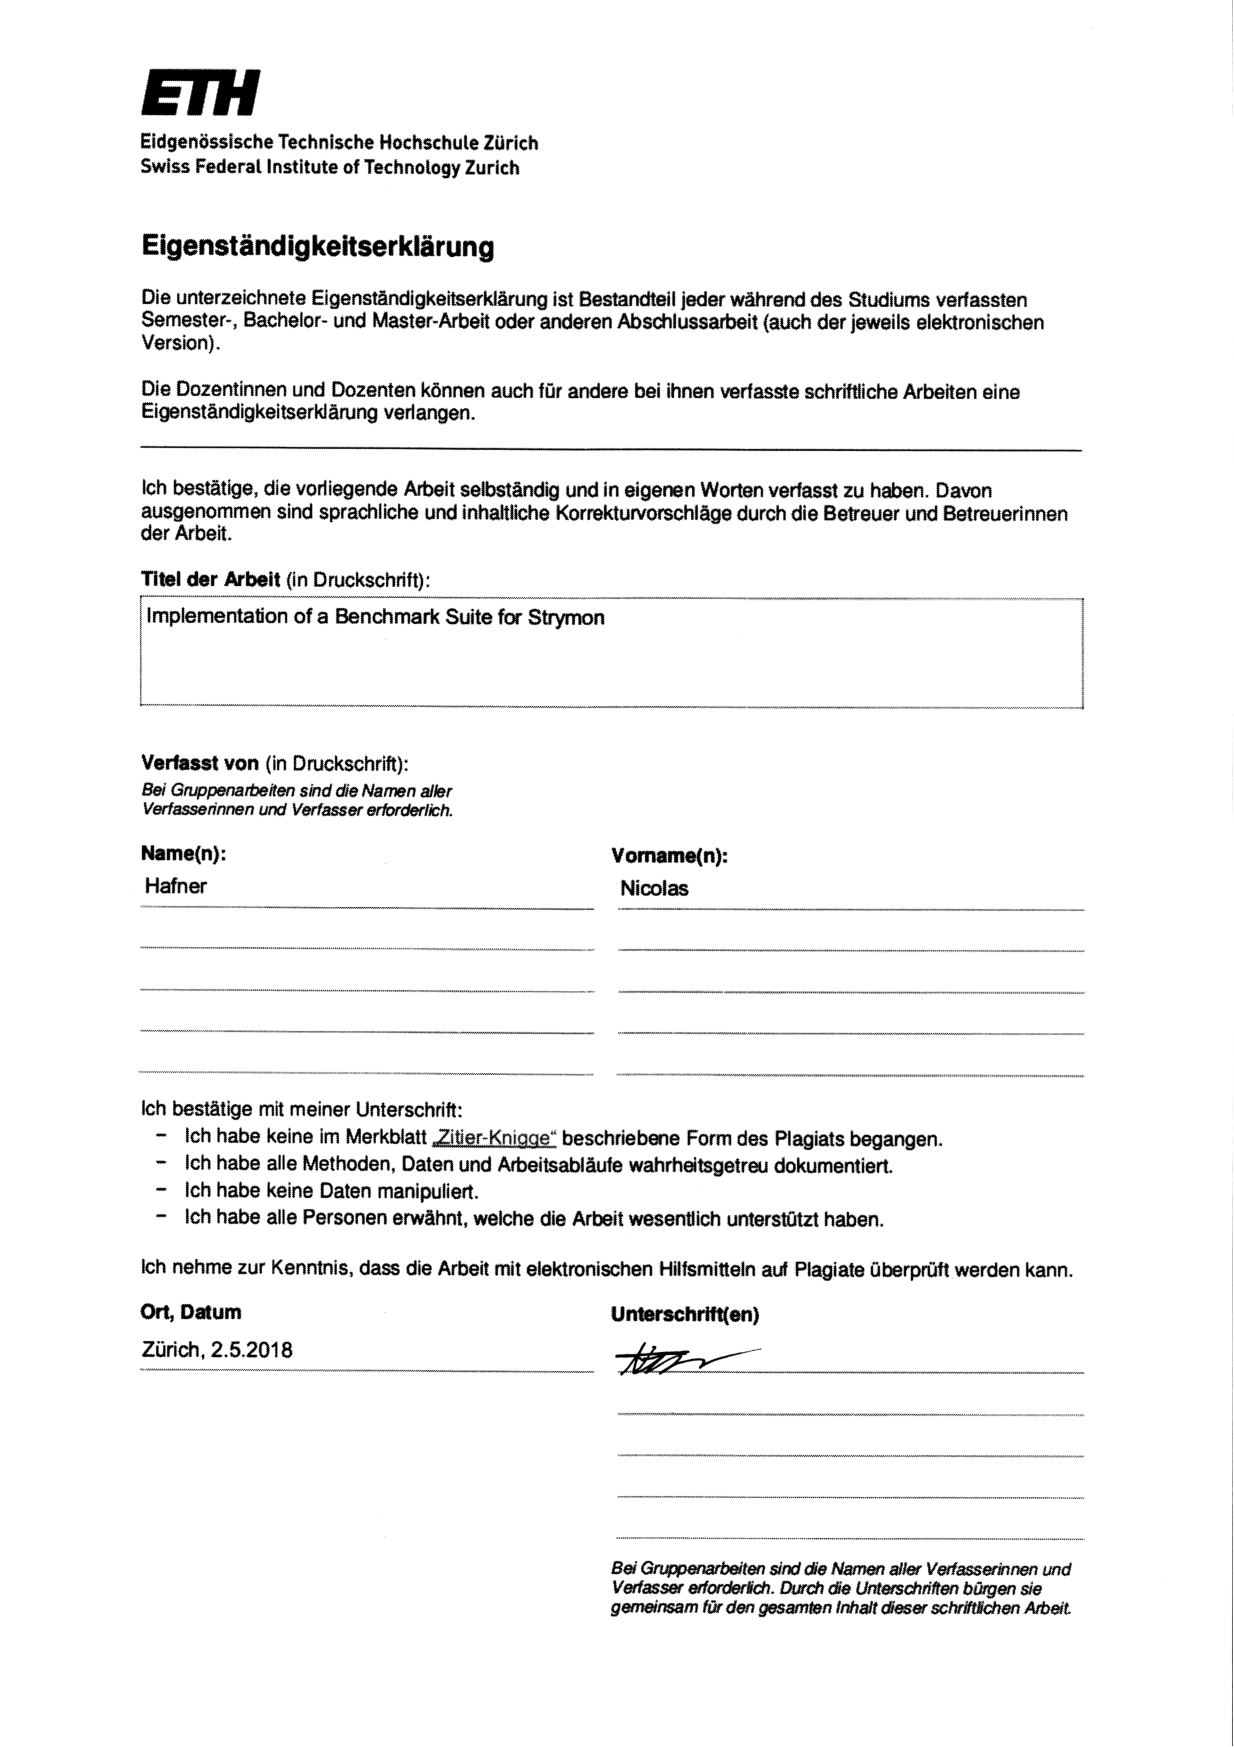
\includepdf{images/independence-declaration.pdf}
\end{document}
%%% Local Variables:
%%% mode: latex
%%% TeX-engine: luatex
%%% TeX-master: t
%%% TeX-command-extra-options: "-shell-escape"
%%% End:
